\chapter{Results and Discussion}

\section{Training Dynamics and Convergence}

\section{Qualitative Analysis of Latent Rollouts}

\begin{figure}
	\begin{center}
		\begin{subfigure}{0.45\textwidth}
			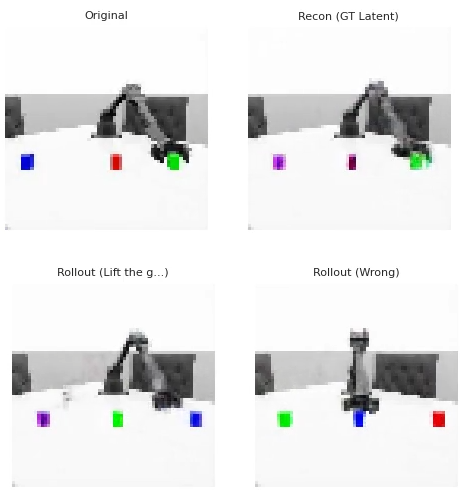
\includegraphics[width=\textwidth]{figures/results/success-decoded.png}
			\caption{}
		\end{subfigure}
		\hfill
		\begin{subfigure}{0.45\textwidth}
			
\includegraphics[width=\textwidth]{figures/results/results-video_qr.pdf}
			\caption{}
		\end{subfigure}
	\end{center}
	\caption{\textbf{Qualitative Visualization of Latent Reasoning.}\ (a) A frame from the video syncing together the ground truth video, the reconstructed frames from \cref{eq:reconst_obs}, decoded latent rollouts from \cref{eq:open_ro_correct} and \cref{eq:open_ro_wrong}, (b) QR code to view the video on Google Drive}
	\label{fig:qual_vis}
\end{figure}


\section{Quantitative Task Sensitivity}

\section{Latent Manifold Analysis}

